\section{Directed Team Graph (DiTG)}

As described in the previous section, we modeled a WiSAR team as a collection of Mealy machines, called {\em actors}, augmented with a simple form of memory.  A key element of these actors is that inputs to one actor can be outputs from another actor.  We can therefore create a directed graph from actor to actor, with an edge from actor~A to actor~B existing if the output from actor~A is a possible input to actor~B.  We call this graph a {\em Directed Team Graph} (DiTG); Figure~\ref{fig:ditg} illustrates the DiTG for the WiSAR team used in this paper.   

\subsection{Labeled Edges}
Using the fact that multiple resource theory \cite{wickens2002multiple} indicates that visual and auditory channels can be perceived in parallel, it is useful to label the edges in the graph with the a {\em channel type} as in Figure~\ref{fig:ditg_detail}).  These labels allow the model-checker to identify when multiple signals are given to a single actor over the same channel.  When this occurs, we expect actor workload to be high.

%We hope to gain
%insight into decreasing the system workload, and possibly combining roles, by
%establishing metrics associated with the system model and model simulation. 
%These metrics can then be used to determine if changes to the model represent a
%decrease in operator workload.

\begin{figure}[hbt]
\center
\setlength{\abovecaptionskip}{1mm}
\setlength{\belowcaptionskip}{1mm}
\setlength{\textfloatsep}{1mm}
\setlength{\floatsep}{1mm}
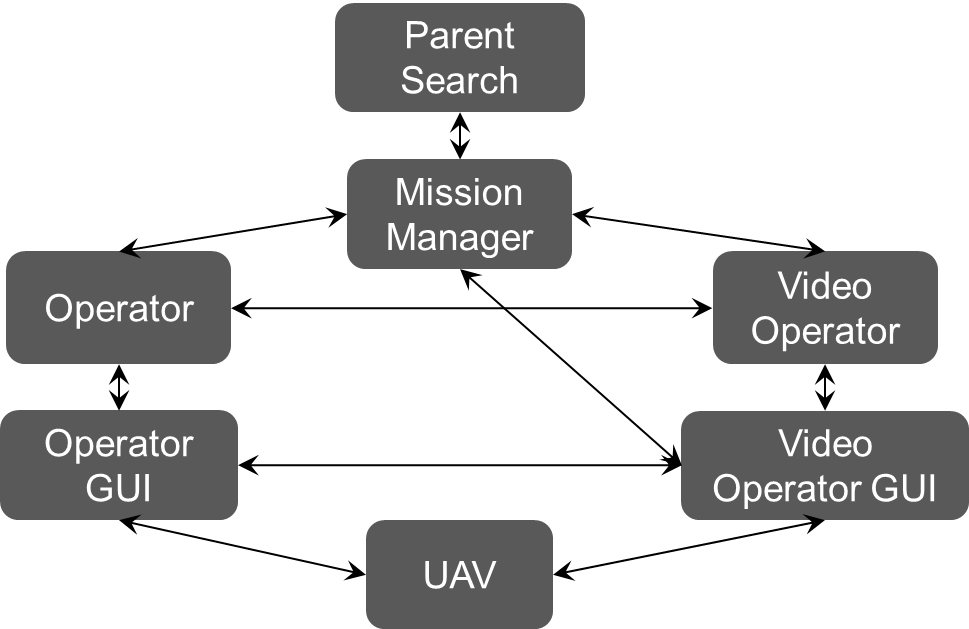
\includegraphics[height=2in]{ditg.png}
\caption{High Level DiTG}
\label{fig:ditg}
\end{figure}

\begin{figure}[hbt]
\center
\setlength{\abovecaptionskip}{1mm}
\setlength{\belowcaptionskip}{1mm}
\setlength{\textfloatsep}{1mm}
\setlength{\floatsep}{1mm}
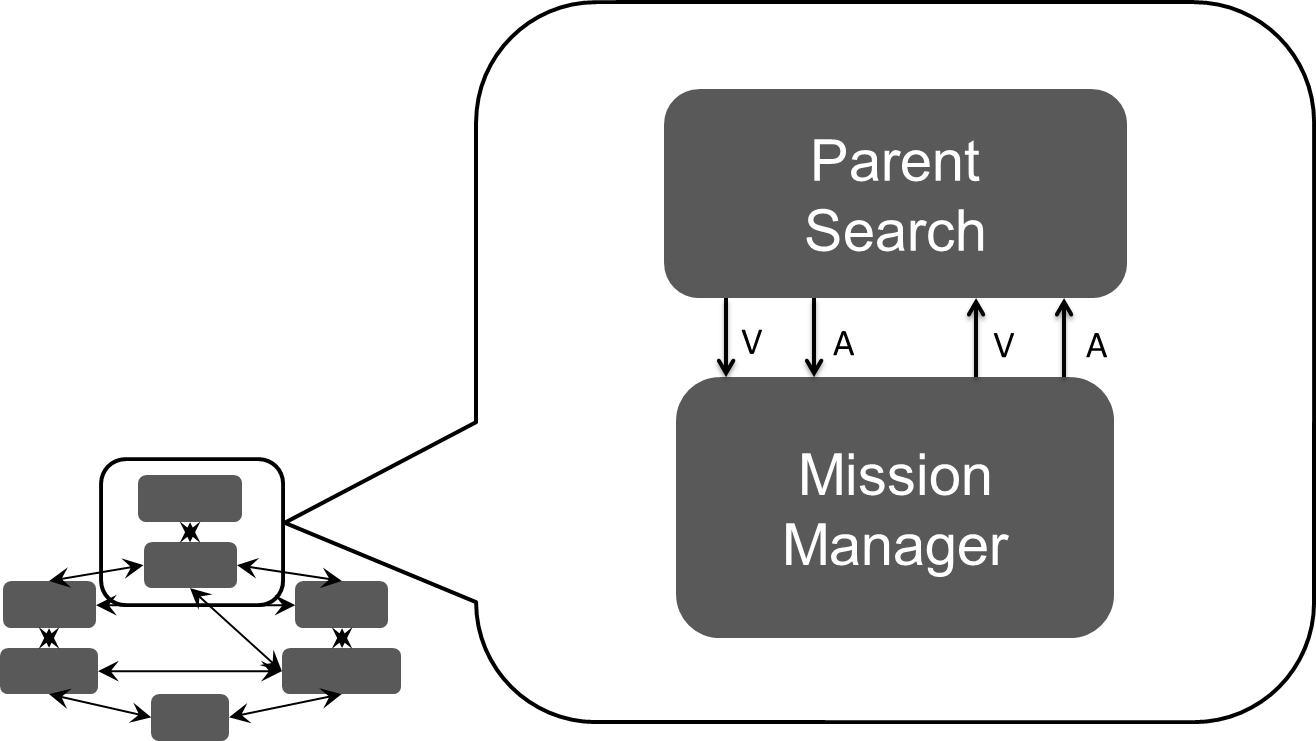
\includegraphics[height=1.9in]{ditg_detailed.png}
\caption{Detail view of DiTG: V is a Visual channel and A is an Audio channel}
\label{fig:ditg_detail}
\end{figure}

%Formally, the framework is the following mathematical structures:
% \begin{equation}
% 	DiTG = (A, \Phi, \forall a_i \in A~ \exists \Phi_i \subset \Phi)
% \end{equation}

% \begin{equation}
% 	Actor = (S, s_0, s_{current}, \Omega_A, \Sigma_A \subset \Phi, \Lambda_A
% 	\subset \Phi)
 %\label{eq:actor}
 %\end{equation}
%
% \begin{equation}
%	State = (T_{enabled}, T_{disabled}) : T_{enabled} \cap T_{disabled} = \emptyset
% \label{eq:state}
%\end{equation}
%
%\begin{equation}
%\begin{split}
%	Transition = (\Omega_{input} \subset \Omega_A, \Sigma_{input} \subset \Sigma_A,\\
%	\Omega_{value}^{input}, \Sigma_{value}^{input} \\
%	\Omega_{output} \subset \Omega_A, \Lambda_{output} \subset \Lambda_A, \\
%	\Omega_{value}^{output}, \Lambda_{value}^{output}, duration)
% \label{eq:transition}
% \end{split}
%\end{equation}

%\begin{equation}
%\begin{split}
%Channel (\phi) = (type \in (visual, audio), \\
%value \in (null, *), 
% a_i^{source}, a_j^{target}) : i \neq j
% \label{eq:channel}
% \end{split}
%\end{equation}
%
%\begin{equation}
%Declarative Memory(\omega) = value \in (null, *)
%\end{equation}


%\noindent where $A$ is a set of actors, $S$ a set of
%states, $T$ a set of transitions, $\Phi$ a set of channels, $\Omega$ a set of
%declarative memory, $\Sigma$ a set of input channels, and $\Lambda$ a set of
%output channels.



\subsection{Overview of Implementation}
We represent a system as a DiTG, a collection of
actors connected to one another by a set of channels.  Whenever the state of the
system changes, an actor will petition from its current state, a list of enabled
transitions thus defining what decisions can be made.  The actor may then
activate one of these transitions.  

Because transitions from one state to another take time, as encoded in the {\em Duration} element of the output, it is useful to label transitions as either {\em active} or {\em fired}.  Note that when we presented the model of an actor, we labeled transitions as {\em enabled} and {\em disabled}, which was sufficient when we considered the actor in isolation.  When we consider the workload of an actor as part of the overall team, workload depends on what is going on with other team members, so we have added the active and fired labels to so that we can determine when an enabled transition (meaning a possible choice available to an actor) is chosen by an actor (making it active) and when the actor completes the work required to produce the next state (the transition fires).  

From an implementation perspective, when a transition becomes active it creates temporary
output values for declarative memory and channels.  These temporary values are
then applied to the actual declarative memory and channel values once the transition fires.

\subsection{Actor vs Tasks}
For our model we never explicitly define a single task.  Instead
we define actors, states, and transitions.  Each transition defines its own
perceptual, cognitive, response, and declarative resources \cite{salvucci2008threaded}, allowing the model to represent multiple possible tasks.  In this way, an actor's state
determines what task(s) are being performed, achieving multi-tasking without
explicitly defining tasks. 

%\subsection{Model Creation}
%To simplify the modeling process and ensure rigorous model creation we
%developed a transition language, similar to a Kripke structure, which allows
%models to be expressed as a list of Actor transitions.  A parser then
%automatically generates the classes required to run the model simulation.
%The transition language uses the following structure.
%\begin{equation}
%\begin{split}
%(s_{current}, [\phi_{input} = value,\ldots], [\omega_{input} = value,\ldots],\\
%duration) \times \\
%(s_{next}, [\phi_{output} =
%value,\ldots], [\omega_{output} = value,\ldots])
%\end{split}
%\end{equation}
%\noindent The language is compiled to a Java program suitable to run standalone
%as a simulation or analyzed by the JPF model checker to create
%workload profiles.
=======
\subsection{Model Creation}
To simplify the modeling process and ensure rigorous model creation we
developed a transition language, similar to a Kripke structure, which allows
models to be expressed as a list of Actor transitions.  A parser then
automatically generates the classes required to run the model simulation.
The transition language uses the following structure.
\begin{equation}
\begin{split}
(s_{current}, [\phi_{input} = value,\ldots], [\omega_{input} = value,\ldots],\\
duration) \times \\
(s_{next}, [\phi_{output} =
value,\ldots], [\omega_{output} = value,\ldots])
\end{split}
\end{equation}
\noindent The language is compiled to a Java program suitable to run standalone
as a simulation or analyzed by the JPF model checker to create
workload profiles.
